\section{Android}
Esta sección tiene objetivo presentar las principales características en el desarrollo de la aplicación para Android.
\subsection{Arquitectura de la aplicación}
Para el desarrollo de la aplicación se implemento la arquitectura Clean, la cual como ya se ha mencionado antes se ha mencionado se ha vuelto muy popular en el desarrollo de aplicaciones móviles para android debido a que es una solución que produce sistemas que presentan las siguientes características.

\begin{itemize}
    \item Escalables, por lo que se pueden agregar más funcionalidades de forma sencilla.
    \item Presentan modularidad.
    \item Presentan independencia en cuanto a frameworks, interfaz de usuario y bases de datos.
    \item El proyecto es más fácil de mantener por lo que es más sencillo hacer cambios.
\end{itemize}

Al utilizar esta arquitectura el proyecto queda separado en tres capas como se observa en la figura \ref{fig:capas-arquitectura} con lo cual cada una de ellas tiene su propósito definido.

\begin{figure}[h]
    \centering
    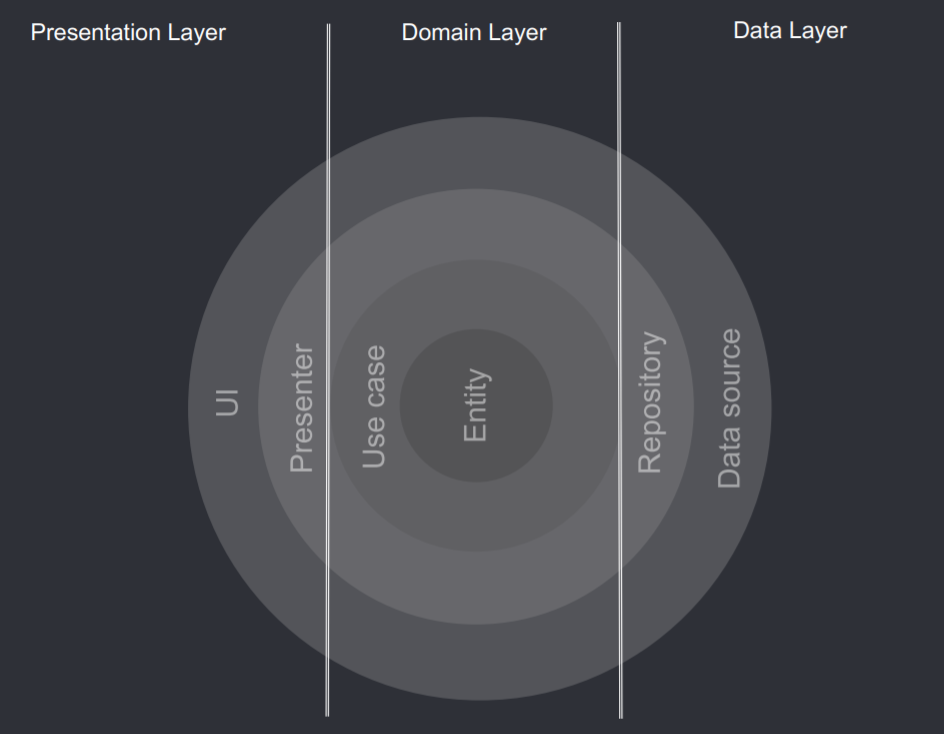
\includegraphics[width=250px]{capitulo5/android/img/capas-clean.png}
    \caption{Tres capas que se tienen al utilizar la arquitectura Clean \cite{cleanGuide}}
    \label{fig:capas-arquitectura}
\end{figure}

\subsubsection{Capa de datos}
La información que se utiliza en el resto de capas proviene de esta capa. Esta capa a su vez se encuentra dividida en la capa de repositorio y en la capa de fuente de datos. 

\paragraph{Capa de repositorio} En esta capa se utiliza el patrón de repositorio como se muestra en la figura \ref{fig:capa-datos}. Gracias a este patrón se puede tener acceso a diferentes fuentes de datos que se encuentran en la capa más baja de nuestra arquitectura, esto nos permite un acceso a los datos de forma transparente para el usuario bajo las condiciones que se presenten.

La forma de utilizar este patrón en la aplicación desarrollado crear una clase en la cual se hace uso de la interfaz que se tiene para el acceso a la fuente de datos. En el siguiente código se puede apreciar el como se crea una instancia de APIService que es nuestra interfaz para fuente de datos.

Después, en nuestro método findAllProyecttosByUser se recupera la información necesaria para mandarla a las capas superiores.

\lstinputlisting[language=Java]{capitulo5/android/src/repositorio.java}

\begin{figure}[h]
    \centering
    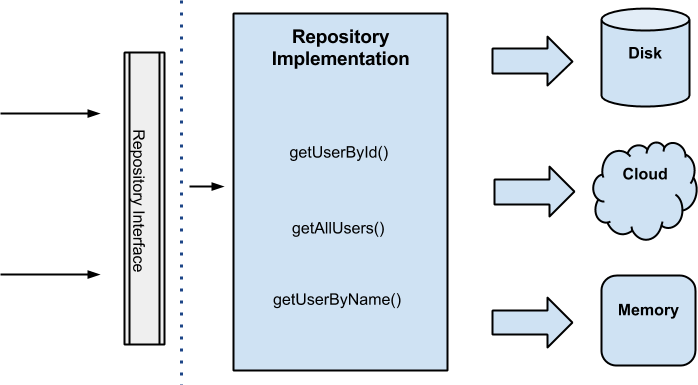
\includegraphics[width=400px]{capitulo5/android/img/capa-datos.png}
    \caption{Capa de datos \cite{cleanWay}}
    \label{fig:capa-datos}
\end{figure}

\paragraph{Capa de fuente de datos} En este trabajo, la fuente de datos que se tiene es un API REST, sin embargo si se requiere acceder a información que se persista en el teléfono se pude agregar otra fuente de datos. Se utilizó retrofit para poder realizar la comunicación con el API REST. 

La forma de utilizar retrofit es crear una interfaz con todos los métodos para recuperar o enviar información al API REST, en esta interfaz cada método tiene la URL a la cual se realizara la petición con alguno de los métodos que tiene HTTP, se tienen los parámetro que se envían y cada método nos regresa una llamada asíncrona que se trabaja en la capa de repositorio. Esto se puede apreciar en el siguiente código.

\lstinputlisting[language=Java]{capitulo5/android/src/APIService.java}

Para poder hacer uso de esta interfaz se tiene que configurar bajo ciertas características especificas como lo son la URL a la cual hará peticiones, el logger que se utilizara para poder observar las peticiones que se realizan y brindar una retroalimentación a la hora de hacer pruebas y por ultimo el parser que se utilizara para trabajar y pasar de clases a datos que el API REST entienda y pueda utilizar, en este caso se utilizo el formato JSON. La definición de estas características se tiene en el siguiente código.

\lstinputlisting[language=Java]{capitulo5/android/src/ServiceGenerator.java}

Finalmente, en esta capa se tienen clases Java que después se mapean a objetos JSON y viceversa, para realizar esto se crea un POJO con los atributos que se necesitan además de agregar anotaciones de retrofit para que el parser pude hacer la conversión necesaria. Un ejemplo de esto es en la siguiente clase de java.

\lstinputlisting[language=Java]{capitulo5/android/src/UsuarioData.java}


\subsubsection{Capa de dominio}
En esta capa es la intermediaria entre las otras dos capas que se tienen, es donde se encuentran los casos de uso también conocidos como interactors como se muestra en la figura \ref{fig:capa-dominio} en ellos la lógica del negocio es ejecutada es por esto que es el núcleo de la aplicación.

Es importante mencionar que esta capa, al ser la encargada del negocio es donde se hacen validaciones en la información y dicha información se adapta para que sea trabajada en la capa de presentación o en la de datos

Además de contener los casos de uso en esta capa se encuentran las entidades y se hace uso de los repositorios para acceder a la información proporcionada por la capa de datos.

\begin{figure}[h]
    \centering
    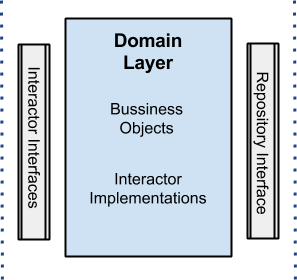
\includegraphics[width=200px]{capitulo5/android/img/capa-dominio.png}
    \caption{Capa de dominio \cite{cleanWay}}
    \label{fig:capa-dominio}
\end{figure}

Para tener un control sobre posibles errores en la capa de presentación o en la capa de datos se utilizan códigos de resultados al igual que una clase que contiene el resultado que se puede presentar, así como la información que se le regresa a la capa de presentación. Se hace uso de genéricos para poder reutilizar esta clase en toda la aplicación y no duplicar código. La clase es la siguiente.

\lstinputlisting[language=Java]{capitulo5/android/src/BusinessResult.java}

La forma en la que se utiliza esta clase en un caso de uso se presenta en el siguiente código que permite iniciar sesión.

\lstinputlisting[language=Java]{capitulo5/android/src/UserInteractorImpl.java}

A su vez el caso de uso utiliza sus propios clases de java para presentar información al usuario en la capa de presentación así como controlar posibles errores en la información que ingrese el usuario los campos de los formularios, un ejemplo de este tipo de clases es el siguiente.

\lstinputlisting[language=Java]{capitulo5/android/src/UsuarioModel.java}

\subsubsection{Capa de presentación}
En esta capa como se muestra en la figura \ref{fig:capa-presentacion} se trabaja con la lógica relacionada a las interfaces que se tienen en la aplicación, es decir a actividades, fragmentos y archivos XML.

\begin{figure}[h]
    \centering
    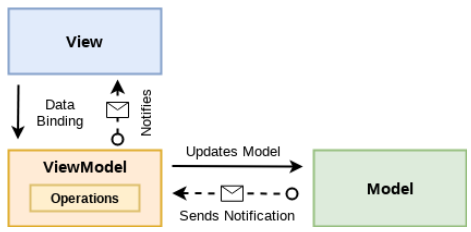
\includegraphics[width=300px]{capitulo5/android/img/capa-presentacion.png}
    \caption{Capa de presentación \cite{cleanWayReload}}
    \label{fig:capa-presentacion}
\end{figure}

En esta capa se pueden trabajar con patrones como MVC y MVP pero en este caso se utiliza el patrón MVVM cada uno con una función en particular. \cite{cleanWayReload}

\begin{itemize}
    \item \textbf{Modelo} Se encarga de representar la información que sera presentada en la vista.
    \item \textbf{Vista} Compuesta en este caso por las actividades y fragmentos de la aplicación, su tarea es mostrar la información, hacen uso de los viewmodels para poder realizar cambios en la interfaz.
    \item \textbf{ViewModel} El ViewModel sera el encargado de ejecutar los casos de uso o interactors con el objetivo de actualizar la vista de acuerdo a la información que presente el modelo.
\end{itemize}


